\documentclass[11pt]{article} 
\usepackage[margin=1in]{geometry} 
\usepackage{wrapfig, amsmath,amsthm,amssymb, graphicx, multicol, array,seqsplit}
\usepackage{microtype,numprint}
\usepackage{siunitx}
\usepackage{paracol}
\usepackage{blkarray,multirow,multicol,booktabs,nicematrix,varwidth}
\usepackage{hhline}
\usepackage{xfrac}
\usepackage[dvipsnames]{xcolor}
\usepackage[makeroom]{cancel}
\usepackage{listings}
\usepackage{mathtools}
\usepackage{tikz,tkz-euclide} 
\usetikzlibrary{intersections,calc,angles}
\setlength{\tabcolsep}{0pt}

\newtheorem{theorem}{Theorem}
\newtheorem{lemma}[theorem]{Lemma}
\NiceMatrixOptions{cell-space-limits = 1pt}

\newcommand{\N}{\mathbb{N}}
\newcommand{\Z}{\mathbb{Z}}
\newcommand{\F}{\mathbb{F}}
\newcommand{\R}{\mathbb{R}}
\newcommand{\C}{\mathbb{C}}
\newcommand{\Q}{\mathbb{Q}}
\newcommand{\bline}{\noindent\rule[0.5ex]{\linewidth}{1pt}}
\newcommand{\ndiv}{\nmid}
\newcommand{\nequiv}{\not\equiv}
\newcommand\leg[2]{\left(\frac{#1}{#2}\right)}


\definecolor{codegreen}{rgb}{0,0.6,0}
\definecolor{codegray}{rgb}{0.5,0.5,0.5}
\definecolor{codepurple}{rgb}{0.58,0,0.82}
\definecolor{backcolour}{rgb}{0.95,0.95,0.92}

%Code listing style named "mystyle"
\lstdefinestyle{mystyle}{
  backgroundcolor=\color{backcolour}, commentstyle=\color{codegreen},
  keywordstyle=\color{magenta},
  numberstyle=\tiny\color{codegray},
  stringstyle=\color{codepurple},
  basicstyle=\ttfamily\footnotesize,
  breakatwhitespace=false,         
  breaklines=true,                 
  captionpos=b,                    
  keepspaces=true,                 
  numbers=left,                    
  numbersep=5pt,                  
  showspaces=false,                
  showstringspaces=false,
  showtabs=false,                  
  tabsize=2
}

%"mystyle" code listing set
\lstset{style=mystyle}

 \newcommand\foo[2]{%
    \begin{minipage}{#1}
    \seqsplit{#2}
    \end{minipage}
    }
\newenvironment{myproof}[1][\proofname]{%
  \begin{proof}[#1]$ $\par\nobreak\ignorespaces
}{%
  \end{proof}
}
\newenvironment{problem}[2][Problem]{\begin{trivlist}
\item[\hskip \labelsep {\bfseries #1}\hskip \labelsep {\bfseries #2.}]}{\end{trivlist}}

\newenvironment{myproblem}[1][Problem]{\begin{trivlist}
    \item[\hskip \labelsep {\bfseries #1.}]}{\end{trivlist}}

\newenvironment{solution}
  {\renewcommand\qedsymbol{$~$}\begin{proof}[Solution]$ $\par\nobreak\ignorespaces}
  {\end{proof}}



\begin{document}

\title{Homework 5}
\author{Rebekah Mayne\\
  Math 370, Fall 2024}
\maketitle


\section{(Page 133-134)}

\begin{problem}{2}
Find a fundamental Pythagorean triangle with hypotenuse 265.
\end{problem}

\begin{solution}
  To get hypotenuse 265, we want to find relatively prime $u$ and $v$ where $u^2+v^2=265$, we can see that $144+121=265$, so we can use $u=12$ and $v=11$. So we have $a=2\cdot 12\cdot 11$, or $a=264$, and $b=12^2-11^2$ or $b=23$. So our triple is 23-264-265.
\end{solution}


\begin{problem}{3}
Find a fundamental Pythagorean triangle with leg 100.
\end{problem}

\begin{solution}
  To get a leg of 100, we can use $2\cdot u\cdot v=100$, and we have $u=25$ and $v=2$. Then our other leg is $25^2-2^2$ or 621, and our hypotenuse of $25^2+2^2$ or 629. So our triple is 100-621-629.
\end{solution}



\begin{problem}{4}
How many Pythagorean triangles (fundamental or not) can you find with hypotenuse 1105?
\end{problem}

\begin{solution}
  We want to start with the PPD, and see that $1105=5\cdot 13\cdot 17$. There is two way for each of these to be split into the sum of two squares. ($2^2+1^2$, $2^2+3^2$, and $4^2+1^2$ and then their respective mirrors), then, there are 3 ways to split these three factors into the two groups that create the sums. So we have 12 possibilities to check for the fundamental triples before we can check for non-fundamental ones.
  For reference we have the sum options as follows:
  \[
    \begin{array}{rl}
      \multirow{2}{*}{$5\cdot 13:$}  & (6+2)^2+(4-3)^2=8^2+1^2      \\
                                     & (3+4)^2+(2-6)^2 = 7^2+4^2    \\
      \multirow{2}{*}{$5\cdot 17:$}  & (4+2)^2+(1-8)^2=6^2+7^2      \\
                                     & (8+1)^2+(2-4)^2 = 9^2+2^2    \\
      \multirow{2}{*}{$13\cdot 17:$} & (7+2)^2+(8-3)^2=9^2+5^2      \\
                                     & (3+8)^2+(2-12)^2 = 11^2+10^2 \\
    \end{array}
  \]

  \begin{center}
    \begin{NiceTabular}[width=0.95\textwidth]{X[l] !{\qquad} X[l]}
      \begin{math}
        \begin{array}[t]{rl}
          \textbf{Option 1:} & (17)(5\cdot 13)       \\
          1105               & =  (4^2+1^2)(8^2+1^2) \\
                             & = (32+1)^2 + (4-8)^2  \\
                             & = 33^2 + 4^2
        \end{array}
      \end{math}

      This means we have $u=33$ and $v=4$, so the legs would be 264 and 1073.

      So we have the pythagorean triangle:
      265-1073-1105

       &
      \begin{math}
        \begin{array}[t]{rl}
          \textbf{Option 2:} & (17)(5\cdot 13)       \\
          1105               & =  (1^2+4^2)(8^2+1^2) \\
                             & = (8+4)^2 + (1-32)^2  \\
                             & = 12^2 + 31^2         \\
        \end{array}
      \end{math}

      This means we have $u=31$ and $v=12$, so the legs would be 744 and 817.

      So we have the pythagorean triangle:
      744-817-1105
      \\
    \end{NiceTabular}
  \end{center}


  \begin{center}
    \begin{NiceTabular}[width=0.95\textwidth]{X[l] !{\qquad} X[l]}
      \begin{math}
        \begin{array}[t]{rl}
          \textbf{Option 3:} & (17)(5\cdot 13)       \\
          1105               & =  (4^2+1^2)(7^2+4^2) \\
                             & = (28+4)^2 + (16-7)^2 \\
                             & = 32^2 + 9^2
        \end{array}
      \end{math}

      This means we have $u=32$ and $v=9$, so the legs would be 576 and 943.

      So we have the pythagorean triangle:
      576-943-1105

       &
      \begin{math}
        \begin{array}[t]{rl}
          \textbf{Option 4:} & (17)(5\cdot 13)       \\
          1105               & =  (1^2+4^2)(7^2+4^2) \\
                             & = (7+16)^2 + (4-28)^2 \\
                             & = 23^2 + 24^2         \\
        \end{array}
      \end{math}

      This means we have $u=24$ and $v=23$, so the legs would be 1104 and 47.

      So we have the pythagorean triangle:
      47-1104-1105

      \\
    \end{NiceTabular}
  \end{center}


  \begin{center}
    \begin{NiceTabular}[width=0.95\textwidth]{X[l] !{\qquad} X[l]}
      \begin{math}
        \begin{array}[t]{rl}
          \textbf{Option 5:} & (13)(5\cdot 17)         \\
          1105               & =  (3^2+2^2)(6^2+7^2)   \\
                             & = (18+14)^2 + (21-12)^2 \\
                             & = 32^2 + 9^2
        \end{array}
      \end{math}

      This means we have $u=32$ and $v=9$, so the legs would be 576 and 943.

      So we have the pythagorean triangle:
      576-943-1105

       &
      \begin{math}
        \begin{array}[t]{rl}
          \textbf{Option 6:} & (13)(5\cdot 17)         \\
          1105               & =  (2^2+3^2)(6^2+7^2)   \\
                             & = (12+21)^2 + (14-18)^2 \\
                             & = 33^2 + 4^2            \\
        \end{array}
      \end{math}

      The triple with $u=33$ and $v=4$ has already been found.
      \\
    \end{NiceTabular}
  \end{center}

  \begin{center}
    \begin{NiceTabular}[width=0.95\textwidth]{X[l] !{\qquad} X[l]}
      \begin{math}
        \begin{array}[t]{rl}
          \textbf{Option 7:} & (13)(5\cdot 17)       \\
          1105               & =  (3^2+2^2)(9^2+2^2) \\
                             & = (27+4)^2 + (6-18)^2 \\
                             & = 31^2 + 12^2
        \end{array}
      \end{math}

      The triple with $u=31$ and $v=12$ has already been found.

       &
      \begin{math}
        \begin{array}[t]{rl}
          \textbf{Option 8:} & (13)(5\cdot 17)       \\
          1105               & =  (2^2+3^2)(9^2+2^2) \\
                             & = (18+6)^2 + (4-27)^2 \\
                             & = 24^2 + 23^2         \\
        \end{array}
      \end{math}
      The triple with $u=24$ and $v=23$ has already been found.

      \\
    \end{NiceTabular}
  \end{center}

  \begin{center}
    \begin{NiceTabular}[width=0.95\textwidth]{X[l] !{\qquad} X[l]}
      \begin{math}
        \begin{array}[t]{rl}
          \textbf{Option 10:} & (5)(13\cdot 17)       \\
          1105                & =  (2^2+1^2)(9^2+5^2) \\
                              & = (18+5)^2 + (10-9)^2 \\
                              & = 23^2 + 1^2
        \end{array}
      \end{math}

      Since both $u=23$ and $v=1$ are odd, it is not a fundamental triple.

       &
      \begin{math}
        \begin{array}[t]{rl}
          \textbf{Option 11:} & (5)(13\cdot 17)       \\
          1105                & =  (1^2+2^2)(9^2+5^2) \\
                              & = (9+10)^2 + (5-18)^2 \\
                              & = 19^2 + 13^2         \\
        \end{array}
      \end{math}

      This means we have $u=19$ and $v=13$, so the legs would be 494 and 192.

      So we have the pythagorean triangle:
      192-494-1105
      \\
    \end{NiceTabular}
  \end{center}

  \begin{center}
    \begin{NiceTabular}[width=0.95\textwidth]{X[l] !{\qquad} X[l]}
      \begin{math}
        \begin{array}[t]{rl}
          \textbf{Option 11:} & (5)(13\cdot 17)         \\
          1105                & =  (2^2+1^2)(11^2+10^2) \\
                              & = (22+10)^2 + (20-11)^2 \\
                              & = 32^2 + 9^2
        \end{array}
      \end{math}

      The triple with $u=32$ and $v=9$ has already been found.


       &
      \begin{math}
        \begin{array}[t]{rl}
          \textbf{Option 12:} & (5)(13\cdot 17)         \\
          1105                & =  (1^2+2^2)(11^2+10^2) \\
                              & = (11+20)^2 + (10-22)^2 \\
                              & = 31^2 + 12^2           \\
        \end{array}
      \end{math}

      The triple with $u=31$ and $v=12$ has already been found.
      \\
    \end{NiceTabular}
  \end{center}
  After this we need to find the possible triples with hypotenuse $5,13,17,5\cdot 13,5\cdot 17,$ and $13\cdot 17$.

  When the hypotenuse is 5 we have $2^2+1^2$, so we have $u=3$ and $v=1$, making the legs, 3 and 4, so we have 3-4-5 or what we want 663-884-1105.

  When the hypotenuse is 13 we have $3^2+2^2$, so we have $u=3$ and $v=2$, making the legs 12 and 5, so we have 5-12-13 or what we want 425-1020-1105.

  When the hypotenuse is 17, we have $4^2+1^2$, so we have $u=4$ and $v=1$, making the legs 8 and 15, so we have 8-15-17, or what we want 520-975-1105.

  When the hypotenuse is $5\cdot 13$, we have two options,
  \begin{center}
    \begin{NiceTabular}[width=0.95\textwidth]{X[l] !{\qquad} X[l]}
      \begin{math}
        \begin{array}[t]{rl}
          \textbf{Option 1:} & 8^2+1^2 \\
        \end{array}
      \end{math}

      Then we have $u=8$ and $v=1$, so our legs are 16 and 63, and we have the triple 272-1071-1105


       &
      \begin{math}
        \begin{array}[t]{rl}
          \textbf{Option 2:} & 7^2+2^2
        \end{array}
      \end{math}

      Then we have $u=7$ and $v=2$, so our legs are 28 and 45, and we have the triple 476-765-1105
      \\
    \end{NiceTabular}
  \end{center}

  When the hypotenuse is $5\cdot 17$, we have two options,
  \begin{center}
    \begin{NiceTabular}[width=0.95\textwidth]{X[l] !{\qquad} X[l]}
      \begin{math}
        \begin{array}[t]{rl}
          \textbf{Option 1:} & 6^2+7^2 \\
        \end{array}
      \end{math}

      Then we have $u=7$ and $v=6$, so our legs are 84 and 13, and we have the triple 169-1092-1105


       &
      \begin{math}
        \begin{array}[t]{rl}
          \textbf{Option 2:} & 9^2+2^2
        \end{array}
      \end{math}

      Then we have $u=9$ and $v=2$, so our legs are 36 and 77, and we have the triple 468-1001-1105
      \\
    \end{NiceTabular}
  \end{center}

  When the hypotenuse is $13\cdot 17$, we have two options,
  \begin{center}
    \begin{NiceTabular}[width=0.95\textwidth]{X[l] !{\qquad} X[l]}
      \begin{math}
        \begin{array}[t]{rl}
          \textbf{Option 1:} & 9^2+5^2 \\
        \end{array}
      \end{math}

      They are both odd, so it is not a triple.


       &
      \begin{math}
        \begin{array}[t]{rl}
          \textbf{Option 2:} & 11^2+10^2
        \end{array}
      \end{math}

      Then we have $u=11$ and $v=10$, so our legs are 220 and 21, and we have the triple 105-1100-1105
      \\
    \end{NiceTabular}
  \end{center}

  Then, all of our representations are as follows
  \begin{multicols}{5}
    \begin{itemize}
      \item $47^2+1104^2$
      \item $105^2+110^2$
      \item $169^2+1092^2$
      \item $192^2+494^2$
      \item $265^2+1073^2$
      \item $272^2+1071^2$
      \item $425^2+1020^2$
      \item $468^2+1001^2$
      \item $476^2+765^2$
      \item $520^2+975^2$
      \item $576^2+943^2$
      \item $663^2+884^2$
      \item $744^2+817^2$
    \end{itemize}
  \end{multicols}

\end{solution}


\begin{problem}{8}
Bhascara(ca. 1150) found a right triangle whose area is numerically equal to the length of its hypotenuse. Show that this cannot happen if the triangle has integer sides.
\end{problem}

\begin{solution}
  Assume to the contrary that we do in fact have a triangle whose area is equal to its hypotenuse, we would then have
  \begin{align*}
    \frac{1}{2} \cdot a \cdot b               & = \sqrt{a^2 + b^2}              \\
    \left(\frac{1}{2}\cdot a \cdot b\right)^2 & = a^2 + b^2                     \\
    \frac{1}{4}\cdot a^2 \cdot b^2            & = a^2 + b^2                     \\
    a^2 \cdot b^2                             & = 4a^2 + b^2                    \\
    a^2                                       & = \frac{4a^2}{b^2} + 1          \\
    1                                         & = \frac{4}{b^2} + \frac{1}{a^2} \\
    1 - \frac{1}{a^2}                         & = \frac{4}{b^2}                 \\
  \end{align*}
  \begin{align*}
    \frac{a^2-1}{a^2} & = \frac{4}{b^2}           \\
    b^2(a^2-1)        & = 4a^2                    \\
    b^2               & = \frac{4a^2}{a^2-1}      \\
    b                 & = \frac{2a}{\sqrt{a^2-1}} \\
  \end{align*}
  For $b$ to be an integer, we need $\sqrt{a^2-1}$ to be an integer, but we know that $a^2$ and $(a+1)^2$ cannot be 1 apart, so $a^2-1$ cannot be a perfect square, and therefore we know $b$ cannot be an integer.
\end{solution}



\begin{problem}{9}
In all of the Pythagorean triangles in the table in the text, one side is a multiple of five. Is this true for all Pythagorean triangles?
\end{problem}

\begin{proof}
  Assume to the contrary that none of the entries in the triple are divisible by 5. We know that all pythagorean triples have the two legs $m\cdot u \cdot v$, and $m(u^2-v^2)$, and hypotenuse $m(u^2+v^2)$. Then, let's look at what squares are mod 5
  \[
    \begin{array}{c|c}
      a & a^2 \pmod{5} \\
      \hline
      0 & 0 \pmod{5}   \\
      1 & 1 \pmod{5}   \\
      2 & -1 \pmod{5}  \\
      3 & -1 \pmod{5}  \\
      4 & 1 \pmod{5}   \\
    \end{array}
  \]
  So we can see that any square must be 0,1, or -1. Then we can see that $u^2+v^2$ is 0, 2 or -2, if it's 0, then one of them is divisible by 5, so both $u$ and $v$ would have to be -1 or 1, but then $u^2-v^2$ will be 0, which is then divisible by 5, so we can see that no matter what one of the sides must be divisible by 5.
\end{proof}



\begin{problem}{10}
Show that 12 divides the product of the legs of a Pythagorean triangle.
\end{problem}

\begin{proof}
  The legs of a pythagorean triangle are always $m(u^2-v^2)$ and $2m\cdot u\cdot v$ for some multiple $m>0$, and $u>v$ that are relatively prime.

  Then let's look mod 4,
  \[
    \begin{array}{c|c}
      a & a^2 \pmod{4} \\
      \hline
      0 & 0 \pmod{4}   \\
      1 & 1 \pmod{4}   \\
      2 & 0 \pmod{4}   \\
      3 & 1 \pmod{4}   \\
    \end{array}
  \]
  Then, we can see that
  \[
    \begin{array}{c|c|c}
      a & b & 2ab \pmod{4} \\
      \hline
      0 & 0 & 0 \pmod{4}   \\
      1 & 0 & 0 \pmod{4}   \\
      2 & 0 & 0 \pmod{4}   \\
      3 & 0 & 0 \pmod{4}   \\
      0 & 1 & 0 \pmod{4}   \\
      1 & 1 & 2 \pmod{4}   \\
      2 & 1 & 0 \pmod{4}   \\
      3 & 1 & 2 \pmod{4}   \\
    \end{array}\;\;\;
    \begin{array}{c|c|c}
      a & b & 2ab \pmod{4} \\
      \hline
      0 & 2 & 0 \pmod{4}   \\
      1 & 2 & 0 \pmod{4}   \\
      2 & 2 & 0 \pmod{4}   \\
      3 & 2 & 0 \pmod{4}   \\
      0 & 3 & 0 \pmod{4}   \\
      1 & 3 & 2 \pmod{4}   \\
      2 & 3 & 0 \pmod{4}   \\
      3 & 3 & 2 \pmod{4}   \\
    \end{array}
  \]
  So we can see they are all divisible by 4, except when both $a$ and $b$ are 1 or 3. So let's look at these in combination, no matter if its 1 or 3, we can see that $a^2-b^2=0$, so then it is also divisible by 4.

  Let's do this again but with mod 3.
  \[
    \begin{array}{c|c}
      a & a^2 \pmod{3} \\
      \hline
      0 & 0 \pmod{3}   \\
      1 & 1 \pmod{3}   \\
      2 & 1 \pmod{3}   \\
    \end{array}
  \]
  Then, we can see that
  \[
    \begin{array}{c|c|c}
      a & b & 2ab \pmod{3} \\
      \hline
      0 & 0 & 0 \pmod{3}   \\
      1 & 0 & 0 \pmod{3}   \\
      2 & 0 & 0 \pmod{3}   \\
      0 & 1 & 0 \pmod{3}   \\
      1 & 1 & 1 \pmod{3}   \\
      2 & 1 & 2 \pmod{3}   \\
      0 & 2 & 0 \pmod{3}   \\
      1 & 2 & 1 \pmod{3}   \\
      2 & 2 & 1 \pmod{3}   \\
    \end{array}
  \]
  So we can see they are all divisible by 3, except when both $a$ and $b$ are 1 or 2. So let's look at these in combination, no matter if its 1 or 2, we can see that $a^2-b^2=0$, so then they are also divisible by 3.
  Since they are both divisible by 4 and 3, this means that it will also be divisible by 12 since $4\bot 3$, so it doesn't overlap.
\end{proof}




\begin{problem}{11}
Show that 60 divides the product of the sides of a Pythagorean triangle.
\end{problem}

\begin{proof}
  By the same logic used in the proof for being divisible by 12, we know that if $a\bot b$ and both $a|n$ and $b|n$, that $ab|n$, since we know 5 divides a side of the triangle, and 12 divides the product of the legs, we know $5\cdot 12=60$ will divide the product of the sides as well.
\end{proof}




\begin{wrapfigure}{R}{0.2\textwidth}
  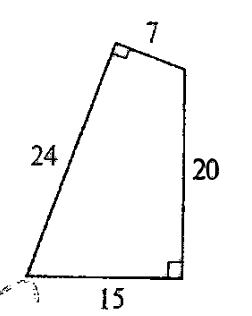
\includegraphics[width=0.65\linewidth]{quad.png}
\end{wrapfigure}


\noindent {\bfseries Problem 12.} Here is a quadrilateral, not a parallelogram, with integer sides and integer area:
\begin{itemize}
  \item [(a)] What is its area?
  \item [(b)] Such quadrilaterals are not common; can you find another?
  \item [(c)] Could you find 1,000,000 more?
\end{itemize}


~\\
\begin{solution}
  \begin{itemize}
    \item [(a)] This quadrilateral can be split down the anti-diagonal into two right triangles, one with sides 7 and 24 and the other with sides 15 and 20. So the area can be found by
          \begin{align*}
            A & = \frac{1}{2}(7)(24) + \frac{1}{2}(15)(20) \\
            A & = 84 + 150                                 \\
            A & = 234
          \end{align*}
    \item [(b)] We could find another set of two triangles that share a hypotenuse by taking two pythagorean triples, and multiplying each by the other's hypotenuse. So let's use 3-4-5 and 12-5-13, and make the hypotenuse 65. Then we have the two triangles 39-52-65 and 60-25-65

          \begin{center}
            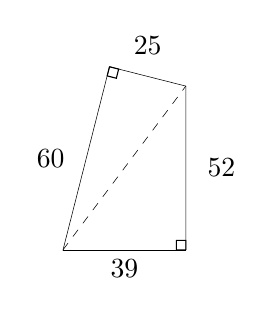
\begin{tikzpicture}[scale=0.04]
              \tkzDefPoint(0,0){A}
              \tkzDefShiftPoint[A](0:39){B}
              \tkzDefShiftPoint[A](53.13:65){C}
              \tkzDefShiftPoint[C](-90-36.87-67.38:25){D}
              \tkzDrawSegments(A,B B,C C,D D,A)
              \tkzDrawSegment[style=dashed](A,C)
              \tkzMarkRightAngles[size=3](A,D,C C,B,A)
              \tkzLabelSegment(A,B){39}
              \tkzLabelSegment[left=1ex](A,D){60}
              \tkzLabelSegment[above=1ex](D,C){25}
              \tkzLabelSegment[right=1ex](B,C){52}

            \end{tikzpicture}
          \end{center}

    \item [(c)] Yes, combining like I did above of two pythagorean triples will continue to work for any combination of them, creating infinitely many possible quadrilaterals.
  \end{itemize}
\end{solution}



\hrule
\section{(Page 148)}

\begin{problem}{1}
Determine which of 1980, 1981, 1982, 1983, and 1984 can be written as a sum of two squares, and for those that can, find a representation.
\end{problem}

\begin{solution}
  \begin{itemize}
    \item 1980: \textcolor{red}{$\times$}
          \begin{align*}
            1980 & = 2^2 \cdot 3^2 \cdot 5 \cdot 11                          \\
                 & = 2^2 \cdot 3^2 \cdot 1 \cdot \textcolor{red}{3} \pmod{4} \\
          \end{align*}
    \item 1981: \textcolor{red}{$\times$}
          \begin{align*}
            1981 & = 7 \cdot 283                           \\
                 & = \textcolor{red}{3} \cdot 283 \pmod{4} \\
          \end{align*}
    \item 1982: \textcolor{red}{$\times$}
          \begin{align*}
            1982 & = 2 \cdot 991                         \\
                 & = 2 \cdot (900 + 80 + 11) \pmod{4}    \\
                 & = 2 \cdot \textcolor{red}{3} \pmod{4} \\
          \end{align*}
    \item 1983: \textcolor{red}{$\times$}
          \begin{align*}
            1982 & = 3 \cdot 661                           \\
                 & = \textcolor{red}{3} \cdot 661 \pmod{4} \\
          \end{align*}
    \item 1984: \textcolor{red}{$\times$}
          \begin{align*}
            1982 & = 2^6 \cdot 31                          \\
                 & = 2^6 \cdot \textcolor{red}{3} \pmod{4} \\
          \end{align*}
  \end{itemize}
\end{solution}


\begin{problem}{2}
Determine which of 2000, 2001, 2002, 2003, and 2004 can be written as a sum of two squares, and for those that can, find a representation.
\end{problem}

\begin{solution}
  \begin{itemize}
    \item 2000: \textcolor{ForestGreen}{$\checkmark$}
          \begin{align*}
            2000 & = 2^4 \cdot 5^3                \\
                 & = 2^4 \cdot 1^3 \pmod{4}       \\
            2000 & = (4^2 + 0^2)\cdot(10^2 + 5^2) \\
                 & = (40+0)^2 + (20-0)^2          \\
            2000 & = 40^2 + 20^2                  \\
          \end{align*}
    \item 2001: \textcolor{red}{$\times$}
          \begin{align*}
            2001 & = 3 \cdot 23 \cdot 29                          \\
                 & = \textcolor{red}{3}\cdot 23 \cdot 29 \pmod{4} \\
          \end{align*}
    \item 2002: \textcolor{red}{$\times$}
          \begin{align*}
            2002 & = 2 \cdot 7 \cdot 11 \cdot 13                                          \\
                 & = 2 \cdot \textcolor{red}{3} \cdot \textcolor{red}{3} \cdot 1 \pmod{4} \\
          \end{align*}
    \item 2003: \textcolor{red}{$\times$}
          \begin{align*}
            2003 & = 2003                        \\
                 & = 2000 + 3 \pmod{4}           \\
                 & = \textcolor{red}{3} \pmod{4} \\
          \end{align*}
    \item 2004: \textcolor{red}{$\times$}
          \begin{align*}
            2004 & = 2^2 \cdot 3 \cdot 167                          \\
                 & = 2^2 \cdot \textcolor{red}{3}\cdot 167 \pmod{4} \\
          \end{align*}
  \end{itemize}
\end{solution}


\begin{lemma}
  $(a^2+b^2)(c^2+d^2)=(ac+bd)^2+(ad-bc)^2$ for any integers $a$, $b$, $c$, and $d$.
\end{lemma}

\begin{problem}{4}
Use Lemma 1 to get two representations of 4453 as a sum of two squares.
\end{problem}

\begin{solution}
  We can see that $4453= 61\cdot 73$, then we can see that $61=5^2+6^2$, and that $73=3^2+8^2$, so two representations would be
  \begin{center}
    \begin{NiceTabular}[width=0.95\textwidth]{X[l] !{\qquad} X[l]}
      \begin{math}
        \begin{array}[t]{rl}
          \textbf{Option 1:} &                       \\
          4453               & = (5^2+6^2)(3^2+8^2)  \\
                             & = (15+48)^2+(40-18)^2 \\
                             & = 63^2 + 22^2         \\
        \end{array}
      \end{math}

      So we can see that $4453=63^2 + 22^2$ is one representation.



       &
      \begin{math}
        \begin{array}[t]{rl}
          \textbf{Option 2:} &                       \\
          4453               & = (6^2+5^2)(3^2+8^2)  \\
                             & = (18+40)^2+(48-15)^2 \\
                             & = 58^2 + 33^2         \\
        \end{array}
      \end{math}

      And that $4453=58^2+33^2$ is another representation.
      \\
    \end{NiceTabular}
  \end{center}
\end{solution}




\begin{problem}{7}
Is it true that if $m$ and $n$ are sums of two squares and $m|n$,then $n/m$ is a sum of two squares? Prove or give a counterexample.
\end{problem}

\begin{proof}
  Let $m,n$ be sums of squares where $m|n$, then we know that for some $k\in \Z$, $km=n$. Then let the expansion of $m$ be $m=a^2+b^2$. So for some $k$, we know that $k(a^2+b^2)=n$ is representable by a sum of two squares.
  Then we can see that $n/m$ is equivalent to $k$.

  If $k$ was not representable by two squares, it would have some odd power of a factor equivalent to $3 \pmod{4}$. But then $n$ would also have an odd power of a factor equivalent to $3\pmod{4}$ unless $a^2+b^2$ also had an odd power of that same factor, however we know this isn't true obviously as it is already in a representation of a sum of two squares.

  Therefore we know $k$ is representable by two squares, and therefore $n/m$ is also a sum of two squares.
\end{proof}


\section{} The following problems are related:

\begin{problem}{(a)}
Prove that if $n\equiv 7\pmod{8}$ then $n$ cannot be expressed as a sum of three squares.
\end{problem}

\begin{proof}
  Look at squares mod 8, we can create a table showing all possible squares.
  \[\begin{array}{c||c|c|c|c|c|c|c|c}
      \begin{matrix}
        a \\
        \hline
        a^2 \pmod{8}
      \end{matrix}
                     &
      \begin{matrix}
        0 \\
        \hline
        0
      \end{matrix} &
      \begin{matrix}
        1 \\
        \hline
        1
      \end{matrix} &
      \begin{matrix}
        2 \\
        \hline
        4
      \end{matrix} &
      \begin{matrix}
        3 \\
        \hline
        1
      \end{matrix} &
      \begin{matrix}
        4 \\
        \hline
        0
      \end{matrix} &
      \begin{matrix}
        5 \\
        \hline
        1
      \end{matrix} &
      \begin{matrix}
        6 \\
        \hline
        4
      \end{matrix} &
      \begin{matrix}
        7 \\
        \hline
        1
      \end{matrix}
    \end{array}\]
  So the only three options are 0, 1, and 4. So then we can look at the possible sums of three squares as follows, WLOG let $a\leq b\leq c\pmod{8}$,
  \[
    \begin{array}{c|c|c| c@{}c}
      a^2 & b^2 & c^2 & a^2 + b^2 + c^2 & \pmod{8} \\
      \hline
      0   & 0   & 0   & 0               & \pmod{8} \\
      0   & 0   & 1   & 1               & \pmod{8} \\
      0   & 0   & 4   & 4               & \pmod{8} \\
      0   & 1   & 1   & 2               & \pmod{8} \\
      0   & 1   & 4   & 5               & \pmod{8} \\
      1   & 1   & 1   & 3               & \pmod{8} \\
      1   & 1   & 4   & 6               & \pmod{8} \\
      1   & 4   & 4   & 1               & \pmod{8} \\
      4   & 4   & 4   & 4               & \pmod{8} \\
    \end{array}
  \]
  So we can see that if $n\equiv 7\pmod{8}$, that there is no way to write $n$ as a sum of three squares.
\end{proof}

\begin{problem}{(b)}
Show that if $4|(x^2+y^2+z^2)$, then $x,y,$ and $z$ are all even.
\end{problem}

\begin{proof}
  Let, $4|(x^2+y^2+z^2)$, then this means that $x^2+y^2+z^2 \equiv 0 \pmod{4}$. Let's look at possible squares mod 4,
  \[\begin{array}{c||c|c|c|c}
      \begin{matrix}
        a \\
        \hline
        a^2 \pmod{8}
      \end{matrix}
                     &
      \begin{matrix}
        0 \\
        \hline
        0
      \end{matrix} &
      \begin{matrix}
        1 \\
        \hline
        1
      \end{matrix} &
      \begin{matrix}
        2 \\
        \hline
        0
      \end{matrix} &
      \begin{matrix}
        3 \\
        \hline
        1
      \end{matrix}
    \end{array}\]
  So the only three options are 0, 1, and those are when $a$ is odd and even respectively. So then we can look at the possible sums of three squares as follows, WLOG let $a\leq b\leq c \pmod{4}$,
  \[
    \begin{array}{c|c|c| c@{}c}
      a^2 & b^2 & c^2 & a^2 + b^2 + c^2 & \pmod{4} \\
      \hline
      0   & 0   & 0   & 0               & \pmod{4} \\
      0   & 0   & 1   & 1               & \pmod{4} \\
      0   & 1   & 1   & 2               & \pmod{4} \\
      1   & 1   & 1   & 3               & \pmod{4} \\
    \end{array}
  \]
  Then, we can see that the only way for $x^2+y^2+z^2\equiv 0 \pmod{4}$ is when $x^2\equiv y^2\equiv z^2\equiv 0 \pmod{4}$, which means that $x,y,z$ must all be even.
\end{proof}


\begin{problem}{(c)}
Use parts (a) and (b) to show that no integer of the form $4^k(8m+7)$ can be written as a sum of three squares.
\end{problem}

\begin{proof}
  Let $n=4^k(8m+7)$. Assume to the contrary that $n$ can be written as a sum of three squares, so $n=a^2+b^2+c^2$.

  Check when $k=0$, then we have $n=8m+7$, and looking mod 8, we see $n\equiv 7\pmod{8}$, then by problem (a) we know that it cannot be written as a sum of three squares, so we have to let $k>0$.
  We can see that then $4|n$, so we know that $a$, $b$, and $c$, are all even. So, we know that $a/2$, $b/2$, and $c/2$ are all integers as well. Then we have
  \[
    \left(\frac{a}{2}\right)^2 + \left(\frac{b}{2}\right)^2 + \left(\frac{c}{2}\right)^2 = 4^{k-1} (8m+7)
  \]
  If we have $k=1$, then we are back to having it be congruent to 7 mod 8, which is not possible, so we know that $k>1$. However, if we have $k>1$, we know that $\sfrac{a}{2},\sfrac{b}{2}, \sfrac{c}{2}$ are all also even, meaning that we could then have
  \[
    \left(\frac{a}{4}\right)^2 + \left(\frac{b}{4}\right)^2 + \left(\frac{c}{4}\right)^2 = 4^{k-2} (8m+7)
  \]
  And we can see that if we have $k=2$, then we are back to having it be congruent to 7 mod 8, which is not possible, so we know that $k>2$.
  So say that we do this until we know that $k=n$ for some $n$, and we have done this process until we know that $k>n-1$ then we have
  \[
    \left(\frac{a}{2^{n}}\right)^2 + \left(\frac{b}{2^{n}}\right)^2 + \left(\frac{c}{2^{n}}\right)^2 = 4^{k-n} (8m+7)
  \]
  And we can see that this means that if we have $k=n$, then we are back to having it be congruent to 7 mod 8, so no matter what $n$ we have this is not possible, because there is no value of $k$ that will every satisfy the conditions.


\end{proof}


\textbf{Important Note:} We have only covered up to page 89 in the  section on Quadratic Congruences so please only use results from the class lecture notes to solve the following problems. Do not use Theorem 4 and beyond (pages 90-92) to solve these problems. We will learn it after we prove it!

~\\
\hrule

\section{} Determine which of the following congruences have solutions. For the ones that have solutions, find them:
\begin{itemize}
  \item [(a)] $x^2\equiv 7 \pmod{53}$
  \item [(b)] $x^2\equiv 14 \pmod{31}$
  \item [(c)] $x^2\equiv 53 \pmod{7}$
  \item [(d)] $x^2\equiv 25 \pmod{997}$
\end{itemize}

\begin{solution}
  \begin{itemize}
    \item [(a)] We want to check if 7 is a QR mod 53, so we can do the following,
          \[
            \begin{array}{r @{\hspace{1pt}} l l}
              7^{26} & \equiv (7^2)^{13}                & \pmod{53} \\
                     & \equiv (-4)^{13}                 & \pmod{53} \\
                     & \equiv (-1)\cdot 4^{13}          & \pmod{53} \\
                     & \equiv (-1)\cdot (4^3)^4 \cdot 4 & \pmod{53} \\
                     & \equiv (-1)\cdot 11^4 \cdot 4    & \pmod{53} \\
                     & \equiv (-1)\cdot 15^2 \cdot 4    & \pmod{53} \\
                     & \equiv (-1)\cdot 13 \cdot 4      & \pmod{53} \\
                     & \equiv (-1)\cdot (-1)            & \pmod{53} \\
              7^{26} & \equiv 1                         & \pmod{53}
            \end{array}
          \]
          So we see that 7 is a QR mod 53, so lets look for a solution
          \[\begin{array}{r @{\hspace{1pt}} l l}
              x^2 & \equiv 7 \equiv 60 \equiv 2^2 \cdot 15    & \pmod{53} \\
              x^2 & \equiv 2^2 \cdot 68  \equiv 2^2 \cdot 121 & \pmod{53} \\
              x^2 & \equiv 2^2 \cdot 11^2                     & \pmod{53} \\
              x   & \equiv 2\cdot 11                          & \pmod{53} \\
              x   & \equiv 22                                 & \pmod{53}
            \end{array}\]
          So our two solutions are $x\equiv 22\pmod{53}$ and $x\equiv 31 \pmod{53}$.
    \item [(b)] We want to check if 14 is a QR mod 31, so we can do the following,
          \[
            \begin{array}{r @{\hspace{1pt}} l l}
              14^{15} & \equiv 7^{15} \cdot (2^5)^3  & \pmod{31} \\
                      & \equiv (7^{3})^5 \cdot (1)^3 & \pmod{31} \\
                      & \equiv (2)^5                 & \pmod{31} \\
              14^{15} & \equiv 1                     & \pmod{31} \\
            \end{array}
          \]
          So we see that 14 is a QR mod 31, so lets look for a solution
          \[\begin{array}{r @{\hspace{1pt}} l l}
              x^2 & \equiv 14 \equiv 45 \equiv 3^2 \cdot 5  & \pmod{31} \\
              x^2 & \equiv 3^2 \cdot 5 \equiv  3^2 \cdot 36 & \pmod{31} \\
              x^2 & \equiv 3^2 \cdot 6^2                    & \pmod{31} \\
              x   & \equiv 3 \cdot 6                        & \pmod{31} \\
              x   & \equiv 18                               & \pmod{31} \\
            \end{array}\]
          So our two solutions are $x\equiv 18\pmod{31}$ and $x\equiv 13 \pmod{31}$.
    \item [(c)] We can see that 53 is a QR mod 997 because $53\equiv 4\pmod{7}$ and 4 is a square generally, so we know that $x\equiv 2 \pmod{7}$ is a solution, so the other solution is $x\equiv 5\pmod{7}$.
    \item [(d)] We can see that 25 is a QR mod 997 because 25 is a square generally, so we know that $x\equiv 5 \pmod{997}$ is a solution, so the other solution is $x\equiv 992\pmod{997}$.
  \end{itemize}
\end{solution}

\hrule

\section{}
\begin{myproblem}
  Find, if they exist, solutions to the following congruences:
  \begin{itemize}
    \item [(a)] $x^2+5x-7\equiv 0 \pmod{19}$
    \item [(b)] $4x^2+6x+1\equiv 0 \pmod{13}$
  \end{itemize}
\end{myproblem}

\begin{solution}
  \begin{itemize}
    \item [(a)] To solve we can do the following
          \[\begin{array}{r @{\hspace{1pt}} l l}
              x^2+5x-7          & \equiv 0   & \pmod{19} \\
              (x^2+24x+144)-151 & \equiv 0   & \pmod{19} \\
              (x+12)^2          & \equiv 151 & \pmod{19} \\
              (x+12)^2          & \equiv -1  & \pmod{19} \\
            \end{array}\]
          We know that since $19\equiv 3 \pmod{4}$ that there is no solution for $y\equiv -1 \pmod{19}$, so there are \textbf{no solutions}.
    \item [(b)] To solve, we want to find what $4^{-1}\pmod{13}$ is, we can see that $4\cdot 10\equiv 1 \pmod{13}$ so $4^{-1}\equiv 10 \pmod{13}$, so then we can do the following
          \[\begin{array}{r @{\hspace{1pt}} l l}
              4x^2+6x+1       & \equiv 0 & \pmod{13} \\
              x^2+60x+10      & \equiv 0 & \pmod{13} \\
              x^2+8x+10       & \equiv 0 & \pmod{13} \\
              (x^2+8x+16) - 6 & \equiv 0 & \pmod{13} \\
              (x+4)^2         & \equiv 6 & \pmod{13} \\
            \end{array}\]
          We want to check if 6 is a QR mod 13, so we can check by follows,
          \[\begin{array}{r @{\hspace{1pt}} l l}
              6^{6} & \equiv (6^2)^3       & \pmod{13} \\
                    & \equiv (-3)^3        & \pmod{13} \\
                    & \equiv -1\cdot (3)^3 & \pmod{13} \\
                    & \equiv -1\cdot 1     & \pmod{13} \\
              6^{6} & \equiv -1            & \pmod{13} \\
            \end{array}\]
          So 6 is a Q-non-R mod 13, so there are \textbf{no solutions}.
  \end{itemize}
\end{solution}



\hrule

\section{}
\begin{myproblem}
  Evaluate the following Legendre symbols:
  \begin{itemize}
    \item [(a)] $\leg{2}{53}$
    \item [(b)] $\leg{52}{53}$
    \item [(c)] $\leg{121}{47}$
  \end{itemize}
\end{myproblem}

\begin{solution}
  \begin{itemize}
    \item [(a)] Let's solve by $\leg{2}{53}\equiv 2^{26} \pmod{53}$,
          \[\begin{array}{r @{\hspace{1pt}} l l}
              \leg{2}{53} & \equiv  2^{26}             & \pmod{53} \\
                          & \equiv (2^6)^{4} \cdot 2^2 & \pmod{53} \\
                          & \equiv (11)^{4} \cdot 2^2  & \pmod{53} \\
                          & \equiv (11^2)^{2} \cdot 4  & \pmod{53} \\
                          & \equiv (15)^{2} \cdot 4    & \pmod{53} \\
                          & \equiv 13 \cdot 4          & \pmod{53} \\
              \leg{2}{53} & \equiv -1                  & \pmod{53} \\
            \end{array}\]
          So we know that $\leg{2}{53}= -1$.
    \item [(b)] We can see that $\leg{52}{53} = \leg{-1}{53}$, since $53 \equiv 1 \pmod{4}$, we know that $\leg{52}{53}=1$.
    \item [(c)] Start with the following
          \begin{align*}
            \leg{121}{47} & = \leg{27}{47}                                     \\
                          & = \leg{-20}{47}                                    \\
                          & = \leg{-1}{47} \cdot \leg{4}{47} \cdot \leg{5}{47} \\
                          & = \leg{-1}{47} \cdot \leg{4}{47} \cdot \leg{5}{47} \\
                          & = -1 \cdot 1 \cdot \leg{5}{47}                     \\
                          & = -1 \cdot \leg{99}{47}                            \\
                          & = -1 \cdot \leg{9}{47} \cdot \leg{11}{47}          \\
                          & = -1 \cdot 1 \cdot 1                               \\
            \leg{121}{47} & = -1
          \end{align*}
          So we know that $\leg{121}{37}= -1$.
  \end{itemize}
\end{solution}


\hrule

\section{}

\textbf{True, False, and Why}

\begin{itemize}
  \item [(a)] Let $n>0$ and $(n,ab)=1$. If neither $x^2\equiv a\pmod{n}$ nor $y^2\equiv b\pmod{n}$ has a solution, then $z^2\equiv ab\pmod{n}$ has a solution.
        \begin{itemize}
          \item[\textbullet]\textbf{True},
                \begin{proof}
                  Let $n>0$ and $(n,ab)=1$. And say that $a$ and $b$ are both Q-non-Rs mod $n$. This means that $a^{\frac{p-1}{2}}\equiv -1 \pmod{n}$ and  $b^{\frac{p-1}{2}}\equiv -1 \pmod{n}$, so then
                  \begin{align*}
                    a^{\frac{p-1}{2}}\cdot b^{\frac{p-1}{2}} & \equiv (-1)\cdot(-1) & \pmod{n} \\
                    a^{\frac{p-1}{2}}\cdot b^{\frac{p-1}{2}} & \equiv 1             & \pmod{n} \\
                    (ab)^{\frac{p-1}{2}}                     & \equiv 1             & \pmod{n} \\
                  \end{align*}
                  This is by definition $ab$ is a QR mod $n$, meaning that $z^2\equiv ab\pmod{n}$ has a solution.
                \end{proof}
        \end{itemize}
  \item [(b)] If $p$ is a prime, $p\equiv 3\pmod{4}$, and $(p,a)=1$, then exactly one of $a$ and $-a$ is a quadratic residue mod $p$.
        \begin{itemize}
          \item[\textbullet]\textbf{True},

                \begin{proof}
                  Let $p$ be a prime, $p\equiv 3\pmod{4}$, and $(p,a)=1$, and WLOG let $a$ be a QR mod $p$, then we know that $a^{\frac{p-1}{2}} \equiv 1 \pmod{p}$, then look at
                  \begin{align*}
                    (-a)^{\frac{p-1}{2}} & \equiv (-1)^{\frac{p-1}{2}} \cdot a^{\frac{p-1}{2}} & \pmod{p} \\
                                         & \equiv (-1)^{\frac{p-1}{2}}                         & \pmod{p} \\
                    \intertext{Since $p\equiv 3\pmod{4}$, $p-1=4k+2$, so $(p-1)/2=2k+1$ so it is odd}
                    (-a)^{\frac{p-1}{2}} & \equiv -1                                           & \pmod{p} \\
                  \end{align*}
                  So $-a$ is a Q-non-R mod $p$.

                  On the other hand, let $p$ be a prime, $p\equiv 3\pmod{4}$, and $(p,a)=1$, and WLOG let $a$ be a Q-non-R mod $p$, then we know that $a^{\frac{p-1}{2}} \equiv -1 \pmod{p}$
                  then look at
                  \begin{align*}
                    (-a)^{\frac{p-1}{2}} & \equiv (-1)^{\frac{p-1}{2}} \cdot a^{\frac{p-1}{2}} & \pmod{p} \\
                                         & \equiv (-1)^{\frac{p-1}{2}} \cdot (-1)              & \pmod{p} \\
                    \intertext{Since $p\equiv 3\pmod{4}$, $p-1=4k+2$, so $(p-1)/2=2k+1$ so it is odd}
                    (-a)^{\frac{p-1}{2}} & \equiv -1  \cdot (-1)                               & \pmod{p} \\
                    (-a)^{\frac{p-1}{2}} & \equiv 1                                            & \pmod{p} \\
                  \end{align*}
                  So $-a$ is a QR mod $p$.

                  Either way, exactly one of $a$ or $-a$ is a quadratic residue mod $p$.
                \end{proof}
        \end{itemize}
\end{itemize}











\end{document}